% Auto-generated by make_all_paper.py -- do not edit.
% Build:  cd latex && latexmk -pdf main.tex
\documentclass[10pt]{article}
% ============================================================================
% Vendored preamble for the HyperMIS reproducibility document (main.tex).
%
% Self-contained snapshot of the packages and macros that the generated
% figure/table fragments depend on, distilled from the paper's paper.tex,
% defs.tex and tikz/tikzdefs.tex.  It lets THIS repository build every
% generated artifact into a single PDF WITHOUT the paper checkout.
%
% It is NOT used by the paper (the paper has its own preamble).  If the
% generated fragments start using a new macro, add it here to keep main.tex
% building.  The plot colours are regenerated (write_plot_colors), everything
% else here is static.
% ============================================================================

\usepackage[a4paper, margin=1.5cm]{geometry}
\usepackage[T1]{fontenc}
\usepackage[utf8]{inputenc}
\usepackage{lmodern}

% --- tables -----------------------------------------------------------------
\usepackage{booktabs}
\usepackage{array}
\usepackage{multirow}
\usepackage{multicol}
\usepackage[table]{xcolor}
\usepackage{graphicx}
\usepackage{adjustbox}      % \resizebox around the wide tables
\usepackage{pdflscape}      % landscape per-instance table (tab:overview)

% --- math -------------------------------------------------------------------
\usepackage{amsmath}
\usepackage{amssymb}
\usepackage{amsfonts}
\usepackage{bm}
\usepackage{mathtools}

% --- numbers ----------------------------------------------------------------
\usepackage{siunitx}
\sisetup{detect-weight=true, detect-inline-weight=math,
         group-separator={\,}, group-minimum-digits=4}
\usepackage{numprint}
\npthousandsep{\,}
\npdecimalsign{.}
\usepackage{xstring}        % \IfStrEqCase inside \rname

% --- references (\nameref is the \rname fallback) ---------------------------
\usepackage{hyperref}

% --- plots ------------------------------------------------------------------
\usepackage{pgf}
\usepackage{pgfplots}
\usepackage{pgfplotstable}
\usepackage{tikz}
\usepgfplotslibrary{colorbrewer, statistics, groupplots}
\usetikzlibrary{arrows.meta, positioning, tikzmark, calc, bending,
                shadows, shapes, patterns}
\pgfplotsset{compat=1.18}
\usepackage{wasysym}        % timeout glyph in the performance profile

% Generated plot colours c<name>, refreshed by write_plot_colors().
% Auto-generated plot colours -- do not edit.
% Source: paper_plot_common.write_plot_colors().
\definecolor{cTime}{RGB}{27,158,119}
\definecolor{cnored}{RGB}{27,158,119}
\definecolor{cred}{RGB}{217,95,2}
\definecolor{ctie}{RGB}{117,112,179}
\definecolor{crecompute}{RGB}{27,158,119}
\definecolor{cprecompute}{RGB}{217,95,2}
\definecolor{condemand}{RGB}{117,112,179}
\definecolor{cnrilp}{RGB}{217,95,2}
\definecolor{cfrilp}{RGB}{231,41,138}
\definecolor{crilp}{RGB}{102,166,30}
\definecolor{cilp}{RGB}{230,171,2}
\definecolor{cgfilp}{RGB}{166,118,29}
\definecolor{cgfrilp}{RGB}{102,102,102}
\definecolor{cstruction}{RGB}{27,158,119}
\definecolor{crstruction}{RGB}{217,95,2}
\definecolor{cbmatching}{RGB}{31,120,180}
\definecolor{crbmatching}{RGB}{227,26,28}
\definecolor{cvcsolver}{RGB}{23,190,207}
\definecolor{crvcsolver}{RGB}{152,78,163}
\definecolor{csatreduce}{RGB}{255,127,0}
\definecolor{crsatreduce}{RGB}{65,105,105}
\definecolor{cgrilp}{RGB}{128,0,38}
% Named DARK2 palette shared with the reduction figures / obs boxes.
\definecolor{d2green}{RGB}{27,158,119}
\definecolor{d2orange}{RGB}{217,95,2}
\definecolor{d2purple}{RGB}{117,112,179}
\definecolor{d2pink}{RGB}{231,41,138}
\definecolor{d2lime}{RGB}{102,166,30}
\definecolor{d2gold}{RGB}{230,171,2}
\definecolor{d2brown}{RGB}{166,118,29}
\definecolor{d2gray}{RGB}{102,102,102}


% ============================================================================
% Macros the fragments reference, copied from the paper's defs.tex.
% ============================================================================
\newcommand{\strong}{\textsc{R}}
\newcommand{\strongeduced}{\strong{}educed}
\newcommand{\ilp}{\textsc{ILP}}
\newcommand{\ilpg}{\textsc{ILP$_G$}}
\newcommand{\satAndReduce}{\textsc{SatAndReduce}}
\newcommand{\weGotYouCovered}{\textsc{WeGotYouCovered}}
\newcommand{\struction}{\textsc{Struction}}
\newcommand{\cfg}[1]{\textsc{#1}}
\newcommand{\bmatching}{\cfg{matching}}
\newcommand{\rmode}[2][]{\strong$_{#2}^{#1}$}
\newcommand{\tred}[1]{\ensuremath{t_{\strong_{#1}}^{\mathrm{red}}}}
\newcommand{\ttot}[1]{\ensuremath{t_{\strong_{#1}}}}
\newcommand{\red}[3][]{\strong$_{#2}^{#1}$-#3}
\definecolor{lightgray}{rgb}{0.86,0.86,0.86}   % shaded rows in tab:overview
% configuration name macros (\c... = solver, prefixed r/f/g variants = reduced)
\newcommand{\cilp}{\ilp}
\newcommand{\crilp}{\red{r}{\ilp}}
\newcommand{\cnrilp}{\red{p}{\ilp}}
\newcommand{\cfrilp}{\red{d}{\ilp}}
\newcommand{\cgfilp}{\ilpg}
\newcommand{\cgfrilp}[1][]{\red[\star]{d}{\ilpg}}
\newcommand{\cgrilp}[1][]{\red[\star]{G}{\ilpg}}
\newcommand{\cstruction}{\struction}
\newcommand{\crstruction}[1][]{\red[\star]{d}{\struction}}
\newcommand{\csatreduce}{\satAndReduce}
\newcommand{\crsatreduce}[1][]{\red[\star]{d}{\satAndReduce}}
\newcommand{\cvcsolver}{\weGotYouCovered}
\newcommand{\crvcsolver}[1][]{\red[\star]{d}{\weGotYouCovered}}
\newcommand{\cbmatching}{\bmatching}
\newcommand{\crbmatching}[1][]{\red[T]{d}{\bmatching}}
}

% Revision markup (fragments usually do not use it, kept for completeness).
\definecolor{revred}{rgb}{0.75,0.05,0.05}
\newcommand{\rev}[1]{\textcolor{revred}{#1}}
\newcommand{\revcolor}{\color{revred}}

% Abbreviated rule names used in the tables.  In the paper these link to the
% reduction definitions; standalone there is no Section 4 to link to, so
% \redlink just typesets the short name (no undefined-reference warnings).
\newcommand{\redlink}[2]{#2}
\DeclareRobustCommand{\rname}[1]{%
  \IfStrEqCase{#1}{%
    {edgesizereduction}{\redlink{#1}{Edge Size}}%
    {degree-one}{\redlink{#1}{Degree-One}}%
    {edgedomreduction}{\redlink{#1}{F.\,Edge Dom.}}%
    {fastdomination}{\redlink{#1}{F.\,Vertex Dom.}}%
    {vertexdomination}{\redlink{#1}{Vertex Dom.}}%
    {twinreduction}{\redlink{#1}{Twins}}%
    {unconfinedreduction}{\redlink{#1}{Unconfined}}%
    {edgedominationgeneral}{\redlink{#1}{Edge Dom.}}%
  }[\texttt{#1}]%
}

\begin{document}
\begin{center}
  {\Large\bfseries HyperMIS -- Reproducible Figures and Tables}\\[3pt]
  \small Generated from \texttt{results/} by \texttt{make\_all\_paper.py}.
\end{center}
\vspace{1em}

\section*{Reduction effect on instance size (tab:reduction\_effect)}
% Auto-generated by the HyperMIS result pipeline -- do not edit.
% Regenerate with: PAPER_ROOT=<paper> python3 make_<script>.py
\begin{table*}[t]
    \centering
    \small
    \caption{Instance properties before ($H$) and after ($H'$) our reduction routine. The first two rows aggregate all $75$ instances; below, we split them into the $18$ \emph{fully reducible} instances, which preprocessing solves outright, and the $57$ \emph{remaining} ones before and after reduction. Columns: vertices $n$, edges $m$, average edge size $\bar e$, average degree $\bar d$, size $|H|$, and the clique-expansion blow-up $b$. We dash $\bar e$, $\bar d$, and $b$ for the all-instance reduced row, as they are undefined on the fully reduced instances.}
    \label{tab:reduction_effect}
    \setlength{\tabcolsep}{5pt}
    \resizebox{\textwidth}{!}{%
    \begin{tabular}{l r@{\,}l r@{\,}l r@{\,}l r@{\,}l c r@{\,}l}
        & \multicolumn{2}{c}{$n$} & \multicolumn{2}{c}{$m$} & \multicolumn{2}{c}{$\bar e$} & \multicolumn{2}{c}{$\bar d$} & $|H|$ & \multicolumn{2}{c}{$b$} \\
        \midrule
        all, $H$ ($75$) & \numprint{402049} & \textcolor{black!55}{$\pm$\,\numprint{572299}} & \numprint{574261} & \textcolor{black!55}{$\pm$\,\numprint{1115181}} & \numprint{21.22} & \textcolor{black!55}{$\pm$\,\numprint{42.25}} & \numprint{27.36} & \textcolor{black!55}{$\pm$\,\numprint{99.16}} & $(2.6\,\textcolor{black!55}{\pm\,3.3})\times 10^{6}$ & \numprint{58.34} & \textcolor{black!55}{$\times$\,\numprint{15.04}} \\
        all, $H'$ ($75$) & \numprint{118565} & \textcolor{black!55}{$\pm$\,\numprint{249321}} & \numprint{135264} & \textcolor{black!55}{$\pm$\,\numprint{354023}} & \multicolumn{2}{c}{--} & \multicolumn{2}{c}{--} & $(0.5\,\textcolor{black!55}{\pm\,0.9})\times 10^{6}$ & \multicolumn{2}{c}{--} \\
        \midrule
        remaining, $H$ ($57$) & \numprint{466804} & \textcolor{black!55}{$\pm$\,\numprint{586282}} & \numprint{735624} & \textcolor{black!55}{$\pm$\,\numprint{1235087}} & \numprint{16.42} & \textcolor{black!55}{$\pm$\,\numprint{30.74}} & \numprint{30.12} & \textcolor{black!55}{$\pm$\,\numprint{112.77}} & $(3.0\,\textcolor{black!55}{\pm\,3.6})\times 10^{6}$ & \numprint{25.11} & \textcolor{black!55}{$\times$\,\numprint{10.25}} \\
        remaining, $H'$ ($57$) & \numprint{156007} & \textcolor{black!55}{$\pm$\,\numprint{275590}} & \numprint{177979} & \textcolor{black!55}{$\pm$\,\numprint{396621}} & \numprint{6.29} & \textcolor{black!55}{$\pm$\,\numprint{8.04}} & \numprint{7.69} & \textcolor{black!55}{$\pm$\,\numprint{17.59}} & $(0.6\,\textcolor{black!55}{\pm\,1.0})\times 10^{6}$ & \numprint{10.73} & \textcolor{black!55}{$\times$\,\numprint{5.73}} \\
        \midrule
        fully reducible, $H$ ($18$) & \numprint{196993} & \textcolor{black!55}{$\pm$\,\numprint{469994}} & \numprint{63279} & \textcolor{black!55}{$\pm$\,\numprint{87579}} & \numprint{36.40} & \textcolor{black!55}{$\pm$\,\numprint{64.37}} & \numprint{18.60} & \textcolor{black!55}{$\pm$\,\numprint{24.44}} & $(1.4\,\textcolor{black!55}{\pm\,1.8})\times 10^{6}$ & \numprint{797.46} & \textcolor{black!55}{$\times$\,\numprint{8.49}} \\
        fully reducible, $H'$ ($18$) & \multicolumn{2}{c}{0} & \multicolumn{2}{c}{0} & \multicolumn{2}{c}{--} & \multicolumn{2}{c}{--} & \numprint{0} & \multicolumn{2}{c}{--} \\
        \bottomrule
    \end{tabular}}
\end{table*}

\clearpage

\section*{Per-rule ablation (tab:ablation)}
% Auto-generated by the HyperMIS result pipeline -- do not edit.
% NOTE: rule names use \rname (abbreviated + linked, see defs.tex), not
% \nameref -- the generator should emit \rname to keep this on regeneration.
% Regenerate with: PAPER_ROOT=<paper> python3 make_<script>.py
\begin{table*}[t]
  \centering \small
  \caption{Per-rule ablation in three parts. An element is a vertex or an edge,
    and the arrows {\color{black!45}$\downarrow$} and {\color{black!45}$\uparrow$}
    mark the better direction. In \emph{single rule} we apply each rule on its
    own and report the fraction of elements left and the time this takes. In
    \emph{all $\setminus$ rule} we run the full pipeline with that one rule
    disabled and report the difference compared to all rules. For the time we
    give the total $\sum \Delta t$ over all $75$ instances, since the effect is
    concentrated on a few large instances. A positive value
    means using the rule saves time. \emph{In pipeline} gives each rule's share
    of the elements removed and of the total reduction time, together with the
    resulting time per removed element.}
  \label{tab:ablation}
  \resizebox{\textwidth}{!}{%
  \begin{tabular}{l r@{\,}l r@{\,}l r@{\,}l S[table-format=-4.0] S[table-format=2.2] S[table-format=2.2] r@{\,}l}
      & \multicolumn{4}{c}{single rule} & \multicolumn{3}{c}{all $\setminus$ rule} & \multicolumn{4}{c}{in pipeline} \\
    \cmidrule(lr){2-5} \cmidrule(lr){6-8} \cmidrule(lr){9-12}
    & \multicolumn{2}{c}{remaining\,\%\,{\color{black!45}$\downarrow$}} & \multicolumn{2}{c}{$t$\,[s]\,{\color{black!45}$\downarrow$}}
         & \multicolumn{2}{c}{$\Delta$\,remaining\,\%} & {$\sum \Delta t$\,[s]}
         & {removed\,\%\,{\color{black!45}$\uparrow$}} & {time\,\%\,{\color{black!45}$\downarrow$}} & \multicolumn{2}{c}{$t$/elem\,[$\mu$s]\,{\color{black!45}$\downarrow$}} \\
    \midrule
    \rname{edgesizereduction} & 96.14 & \textcolor{black!55}{$\pm$\,13.67} & 0.06 & \textcolor{black!55}{$\times$\,4.67} & 0.00 & \textcolor{black!55}{$\pm$\,0.00} & -6 & 25.41 & 2.54 & 0.16 & \textcolor{black!55}{$\times$\,10.94} \\
    \rname{degree-one} & 79.17 & \textcolor{black!55}{$\pm$\,31.86} & 0.07 & \textcolor{black!55}{$\times$\,4.99} & 0.01 & \textcolor{black!55}{$\pm$\,0.09} & 164 & 32.52 & 21.27 & 1.01 & \textcolor{black!55}{$\times$\,5.73} \\
    \rname{edgedomreduction} & 80.65 & \textcolor{black!55}{$\pm$\,22.36} & 0.11 & \textcolor{black!55}{$\times$\,6.44} & 6.90 & \textcolor{black!55}{$\pm$\,15.28} & 63 & 20.41 & 9.86 & 3.81 & \textcolor{black!55}{$\times$\,11.89} \\
    \rname{fastdomination} & 58.38 & \textcolor{black!55}{$\pm$\,34.57} & 0.28 & \textcolor{black!55}{$\times$\,7.52} & 0.00 & \textcolor{black!55}{$\pm$\,0.02} & 738 & 11.75 & 9.39 & 13.99 & \textcolor{black!55}{$\times$\,7.14} \\
    \rname{vertexdomination} & 65.81 & \textcolor{black!55}{$\pm$\,29.46} & 1.65 & \textcolor{black!55}{$\times$\,17.68} & 0.43 & \textcolor{black!55}{$\pm$\,2.42} & -132 & 3.98 & 15.19 & 33.20 & \textcolor{black!55}{$\times$\,11.19} \\
    \rname{twinreduction} & 81.64 & \textcolor{black!55}{$\pm$\,30.31} & 0.89 & \textcolor{black!55}{$\times$\,11.30} & 0.30 & \textcolor{black!55}{$\pm$\,1.72} & -76 & 0.37 & 4.50 & 76.23 & \textcolor{black!55}{$\times$\,6.09} \\
    \rname{unconfinedreduction} & 45.21 & \textcolor{black!55}{$\pm$\,30.23} & 4.04 & \textcolor{black!55}{$\times$\,21.44} & 12.64 & \textcolor{black!55}{$\pm$\,16.40} & -1264 & 5.56 & 37.25 & 122.98 & \textcolor{black!55}{$\times$\,22.69} \\
    \midrule
    \emph{all rules} & 20.65 & \textcolor{black!55}{$\pm$\,22.98} & 0.98 & \textcolor{black!55}{$\times$\,15.21} & \multicolumn{2}{c}{0} & {0} & {100} & {100} & 3.74 & \textcolor{black!55}{$\times$\,6.91} \\
    \bottomrule
  \end{tabular}}
\end{table*}

\clearpage

\section*{Reduction and solving cost per strategy (tab:strategies)}
% Auto-generated by the HyperMIS result pipeline -- do not edit.
% NOTE: tabcolsep reduced by hand to 2.7pt; at 4pt the tabular overflows the
% text width by ~21pt. Keep this if the table is regenerated.
% Regenerate with: PAPER_ROOT=<paper> python3 make_<script>.py
\begin{table*}[t]
  \centering
  \caption{Reduction and solving cost per strategy on solvable instances. The
    arrows {\color{black!45}$\downarrow$} and {\color{black!45}$\uparrow$}
    mark the better direction, and the best value per column is bold.
    \emph{Reduction} gives the configuration \rmode{x}, the remaining
    vertices, the reduction time $t^{\mathrm{red}}$ and the peak memory. A superscript $\star$
    marks clique expansion and $\mathsf{T}$ marks $H^{\mathsf{T}}$.
    \emph{Solving} gives the total number of instances solved and
    \emph{$t$ all}, the run time over all instances with unsolved ones penalised
    at the $3600$\,s limit.
    \emph{Reduction gain} compares each solver with and without our reductions.
    This includes the number of instances solvable due to reductions
    (\emph{\#solved}), \emph{speedup} and \emph{memory} giving run time and
    peak-memory improvement factors on instances each method solves both ways. The
    mutually solved set differs per row, so these three columns are not comparable
    across rows. Blank cells repeat the numbers above.}
  \label{tab:strategies}
  \setlength{\tabcolsep}{2.7pt}\small
  \begin{tabular}{l S[table-format=4.0] S[table-format=2.2] S[table-format=3.2] l S[table-format=2.0] S[table-format=3.2] S[table-format=2.0] S[table-format=1.2] S[table-format=1.2]}
      \multicolumn{4}{c}{reduction} & \multicolumn{3}{c}{solving} & \multicolumn{3}{c}{reduction gain} \\
    \cmidrule(lr){1-4} \cmidrule(lr){5-7} \cmidrule(lr){8-10}
    {\rmode{}} & {remaining\,{\color{black!45}$\downarrow$}} & {$t^{\mathrm{red}}$\,[s]\,{\color{black!45}$\downarrow$}} & {mem\,[MB]\,{\color{black!45}$\downarrow$}}
      & {solver} & {solved\,{\color{black!45}$\uparrow$}} & {$t$ all\,[s]\,{\color{black!45}$\downarrow$}}
      & {\#solved\,{\color{black!45}$\uparrow$}} & {speedup\,{\color{black!45}$\uparrow$}} & {memory\,{\color{black!45}$\uparrow$}} \\
    \midrule
    \rmode{r} & 2944 & 4.52 & {\bfseries 58.54} & \makebox[1em][l]{}\crilp & 47 & 11.34 & 2 & 1.39 & 2.97 \\
    \rmode{p} & 2899 & 4.09 & 203.82 & \makebox[1em][l]{}\cnrilp & 47 & 24.75 & 3 & 0.59 & 0.96 \\
    \rmode{d} & {\bfseries 2899} & {\bfseries 0.99} & 85.32 & \makebox[1em][l]{\tikz[baseline=-0.55ex]{\draw[cfrilp] plot[only marks, mark=*, mark size=1.7pt, mark options={solid, draw=cfrilp, line width=0.6pt, fill=cfrilp}] coordinates {(0,0)};}}\cfrilp & 51 & 6.85 & 6 & 2.29 & 2.80 \\
    \midrule
    \rmode[\mathsf{T}]{d} & {\bfseries 2899} & {\bfseries 0.99} & 85.32 & \makebox[1em][l]{\tikz[baseline=-0.55ex]{\draw[crbmatching] plot[only marks, mark=pentagon*, mark size=1.7pt, mark options={solid, draw=crbmatching, line width=0.6pt, fill=crbmatching}] coordinates {(0,0)};}}\crbmatching[\mathsf{T}] & 51 & 7.03 & 12 & 2.16 & 3.39 \\
    \midrule
    \rmode[\star]{d} & {\bfseries 2899} & {\bfseries 0.99} & 85.32 & \makebox[1em][l]{\tikz[baseline=-0.55ex]{\draw[cgfrilp] plot[only marks, mark=square*, mark size=1.7pt, mark options={solid, draw=cgfrilp, line width=0.6pt, fill=cgfrilp}] coordinates {(0,0)};}}\cgfrilp[\star] & {\bfseries 52} & {\bfseries 6.43} & 16 & 8.14 & 10.84 \\
     & {} & {} & {} & \makebox[1em][l]{\tikz[baseline=-0.55ex]{\draw[crstruction] plot[only marks, mark=triangle*, mark size=1.7pt, mark options={solid, draw=crstruction, line width=0.6pt, fill=crstruction}] coordinates {(0,0)};}}\crstruction[\star] & 30 & 42.57 & 1 & 12.64 & 11.87 \\
     & {} & {} & {} & \makebox[1em][l]{\tikz[baseline=-0.55ex]{\draw[crsatreduce] plot[only marks, mark=diamond*, mark size=1.7pt, mark options={solid, draw=crsatreduce, line width=0.6pt, fill=crsatreduce}] coordinates {(0,0)};}}\crsatreduce[\star] & 30 & 52.16 & 6 & 17.22 & 13.18 \\
     & {} & {} & {} & \makebox[1em][l]{\tikz[baseline=-0.55ex]{\draw[crvcsolver] plot[only marks, mark=triangle*, mark size=1.7pt, mark options={solid, rotate=180, draw=crvcsolver, line width=0.6pt, fill=crvcsolver}] coordinates {(0,0)};}}\crvcsolver[\star] & 32 & 33.22 & 1 & 13.76 & 7.25 \\
    \rmode[\star]{G} & 2917 & 4.61 & 227.14 & \makebox[1em][l]{\tikz[baseline=-0.55ex]{\draw[cgrilp] plot[only marks, mark=square*, mark size=1.7pt, mark options={solid, draw=cgrilp, line width=0.6pt, fill=cgrilp!35}] coordinates {(0,0)};}}\cgrilp[\star] & 49 & 16.99 & 13 & 5.43 & 6.45 \\
    \bottomrule
  \end{tabular}
\end{table*}

\clearpage

\section*{Neighborhood strategies time--memory (fig:neighborhood-mem)}
% Auto-generated by the HyperMIS result pipeline -- do not edit.
% Regenerate with: PAPER_ROOT=<paper> python3 make_<script>.py
\begin{figure}[t]
  \centering
  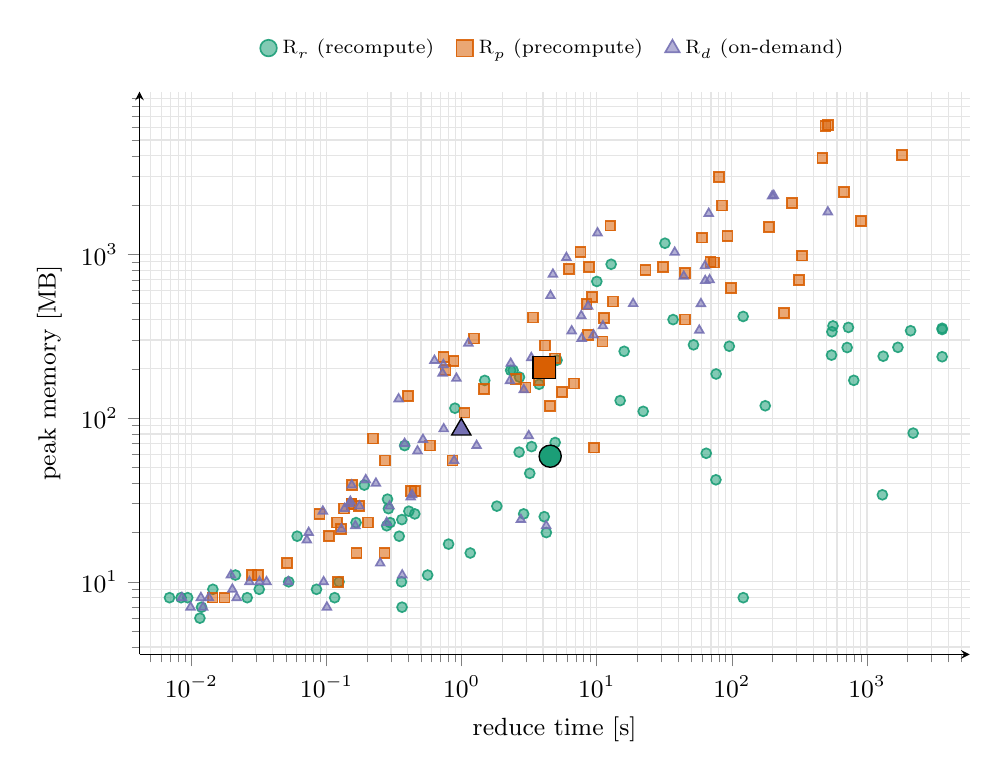
\begin{tikzpicture}
    \begin{axis}[
      width=\linewidth, height=0.72\linewidth,
      scale only axis=false,
      label style={font=\small}, tick label style={font=\small},
      xmode=log, ymode=log,
      xmin=0.004128, xmax=5762, ymin=3.6, ymax=9891,
      xlabel={reduce time [s]}, ylabel={peak memory [MB]},
      legend cell align=left, legend style={at={(0.5,1.04)}, anchor=south, legend columns=-1, draw=none, fill=none, font=\scriptsize, /tikz/every even column/.append style={column sep=6pt}},
      legend image post style={mark size=3pt},
      grid=both, grid style={gray!20}, axis lines=left, tick align=outside,
    ]
      \addplot[only marks, color=crecompute, mark=*, mark size=1.8pt, mark options={solid, draw=crecompute, line width=0.6pt, fill=crecompute, fill opacity=0.55, draw opacity=0.9}] coordinates {(0.5603,11) (1.482,170) (0.00688,8) (2.306,196) (2.877,26) (4.086,25) (3.291,67) (0.2871,28) (0.01441,9) (0.02116,11) (0.01155,6) (0.3588,10) (4.234,20) (0.03175,9) (0.279,22) (550,337) (546.5,242.7) (560.3,366) (798.7,170.2) (76.47,186.1) (713.4,270) (1318,239) (1694,270.7) (729,358.4) (3601,237.2) (1.158,15) (0.00938,8) (0.1148,8) (0.362,7) (0.1237,10) (0.3785,68) (0.08427,9) (1.822,29) (176.6,119) (0.06061,19) (0.0525,10) (64.6,61) (0.01188,7) (0.00838,8) (22.06,110) (0.1653,23) (0.3609,24) (0.2826,32) (0.45,26) (0.4066,27) (0.3451,19) (0.2954,23) (36.71,400) (121.4,8) (5.08,226) (0.8004,17) (10.01,684) (31.96,1171) (12.78,871) (2.679,178) (3.744,161) (2196,81) (1300,34) (76.19,42) (0.8915,115) (2.402,196) (14.9,128) (2103,341.9) (95.71,275) (3601,354) (3601,348) (15.95,256) (121.2,418) (3.191,46) (0.02587,8) (2.663,62) (52,280.5) (0.1904,39) (4.92,71)};
      \addlegendentry{\rmode{r} (recompute)}
      \addplot[only marks, color=cprecompute, mark=square*, mark size=1.8pt, mark options={solid, draw=cprecompute, line width=0.6pt, fill=cprecompute, fill opacity=0.55, draw opacity=0.9}] coordinates {(0.2688,15) (3.387,412) (0.2216,75) (30.97,836) (0.4225,36) (0.4514,36) (11,294) (329.3,983) (4.5,119) (5.521,144) (0.01436,8) (242.3,437) (315.3,699) (0.2028,23) (904.3,1597) (9.255,549) (22.93,806.7) (80.48,2966) (74.11,893.2) (13.25,515.3) (69.56,896.2) (59.94,1266) (92.59,1301) (84.53,1988) (679.4,2409) (0.1195,23) (0.05099,13) (0.02791,11) (0.1212,10) (0.1041,19) (1808,4069) (0.1668,15) (0.2701,55) (4.136,278) (0.8549,55) (277.2,2055) (3.745,171) (0.03094,11) (0.01754,8) (2.528,173) (0.08864,26) (0.1732,29) (0.1546,39) (0.1533,30) (0.1534,30) (0.1281,21) (0.1353,28) (8.751,841) (9.532,66) (4.893,232) (0.5825,68) (6.198,815) (12.6,1499) (7.573,1037) (0.8726,224) (0.7583,197) (467.1,3879) (44.92,773) (6.768,163) (0.4021,137) (0.7343,237) (2.969,154) (188,1470) (11.26,410) (512.9,6182) (494.3,6118) (1.239,306) (8.417,500) (1.05,108) (98.63,623) (4.306,204) (8.606,322.2) (45.06,400) (1.464,151)};
      \addlegendentry{\rmode{p} (precompute)}
      \addplot[only marks, color=condemand, mark=triangle*, mark size=1.8pt, mark options={solid, draw=condemand, line width=0.6pt, fill=condemand, fill opacity=0.55, draw opacity=0.9}] coordinates {(0.2495,13) (0.9146,175) (0.01344,8) (2.307,216) (0.4198,33) (0.4295,34) (0.5171,74) (0.2926,29) (0.02008,9) (0.01959,11) (0.00985,7) (0.3632,11) (4.224,22) (0.03189,10) (0.2787,23) (7.682,422) (18.59,500.7) (37.75,1030) (57.38,344.2) (9.461,322.3) (59.01,500) (44.04,735.9) (68.45,699.7) (63.25,851.4) (513.2,1817) (0.07148,18) (0.01175,8) (0.02687,10) (0.1006,7) (0.03597,10) (0.3784,70) (0.09515,10) (0.2319,40) (3.942,217) (0.07375,20) (0.05208,10) (1.29,68) (0.01219,7) (0.0085,8) (2.276,169) (0.09386,27) (0.1752,29) (0.1537,39) (0.15,31) (0.1476,30) (0.1288,21) (0.1359,28) (4.544,560) (2.743,24) (3.278,234) (0.1634,22) (4.735,757) (10.13,1353) (5.961,957) (0.7325,212) (0.7222,188) (67.4,1780) (6.521,341) (3.137,78) (0.3415,131) (0.6291,225) (2.883,149) (63.47,691.9) (11.1,366) (204.2,2291) (198.6,2276) (1.121,287) (8.617,483) (0.8791,55) (0.02164,8) (0.4712,63) (7.735,306.8) (0.1951,42) (0.7366,86)};
      \addlegendentry{\rmode{d} (on-demand)}
      \addplot[only marks, color=crecompute, mark=*, mark size=4pt, mark options={solid, draw=crecompute, line width=0.6pt, fill=crecompute, draw=black, line width=0.5pt}, forget plot] coordinates {(4.522,58.54)};
      \addplot[only marks, color=cprecompute, mark=square*, mark size=4pt, mark options={solid, draw=cprecompute, line width=0.6pt, fill=cprecompute, draw=black, line width=0.5pt}, forget plot] coordinates {(4.086,203.8)};
      \addplot[only marks, color=condemand, mark=triangle*, mark size=4pt, mark options={solid, draw=condemand, line width=0.6pt, fill=condemand, draw=black, line width=0.5pt}, forget plot] coordinates {(0.994,85.32)};
    \end{axis}
  \end{tikzpicture}
  \caption{Time--memory trade-off of the reduction neighborhood strategies.
    Each small mark is one instance, the large outlined mark is the strategy's
    shifted geometric mean.}
  \label{fig:neighborhood-mem}
\end{figure}

\clearpage

\section*{Performance profiles and cactus plots (fig:solverplots)}
% Auto-generated by the HyperMIS result pipeline -- do not edit.
% Regenerate with: PAPER_ROOT=<paper> python3 make_<script>.py
\begin{figure*}[t]
  \centering
  \centerline{\ref{solverlegend}}
  \vspace{2pt}
  \begin{tikzpicture}
    \begin{axis}[
      width=0.48\linewidth, height=0.32\linewidth,
      xmode=log, log basis x=2,
      xmin=1, ymin=0, ymax=1.02,
      xlabel={$\tau$ (factor from best run time)},
      ylabel={fraction of instances},
      legend cell align=left, legend to name=solverlegend, legend columns=6, legend style={draw=none, fill=none, font=\scriptsize, /tikz/every even column/.append style={column sep=6pt}},
      label style={font=\small}, tick label style={font=\small},
      grid=both, grid style={gray!20}, axis lines=left, tick align=outside,
    ]
    \addplot+[const plot, thick, color=cilp,
             mark=*, mark size=1.6pt, mark options={solid, draw=cilp, line width=0.6pt, fill=white}]
      table[x=tau, y=frac, col sep=tab] {data/plot_data/pp_time_ilp.dat};
    \addlegendentry{\cilp}
    \addplot+[const plot, thick, color=cgfilp,
             mark=square*, mark size=1.6pt, mark options={solid, draw=cgfilp, line width=0.6pt, fill=white}]
      table[x=tau, y=frac, col sep=tab] {data/plot_data/pp_time_gfilp.dat};
    \addlegendentry{\cgfilp}
    \addplot+[const plot, thick, color=cstruction,
             mark=triangle*, mark size=1.6pt, mark options={solid, draw=cstruction, line width=0.6pt, fill=white}]
      table[x=tau, y=frac, col sep=tab] {data/plot_data/pp_time_struction.dat};
    \addlegendentry{\cstruction}
    \addplot+[const plot, thick, color=csatreduce,
             mark=diamond*, mark size=1.6pt, mark options={solid, draw=csatreduce, line width=0.6pt, fill=white}]
      table[x=tau, y=frac, col sep=tab] {data/plot_data/pp_time_satreduce.dat};
    \addlegendentry{\csatreduce}
    \addplot+[const plot, thick, color=cvcsolver,
             mark=triangle*, mark size=1.6pt, mark options={solid, rotate=180, draw=cvcsolver, line width=0.6pt, fill=white}]
      table[x=tau, y=frac, col sep=tab] {data/plot_data/pp_time_vc_solver.dat};
    \addlegendentry{\cvcsolver}
    \addplot+[const plot, thick, color=cbmatching,
             mark=pentagon*, mark size=1.6pt, mark options={solid, draw=cbmatching, line width=0.6pt, fill=white}]
      table[x=tau, y=frac, col sep=tab] {data/plot_data/pp_time_bmatching.dat};
    \addlegendentry{\cbmatching}
    \addplot+[const plot, thick, color=cfrilp,
             mark=*, mark size=1.6pt, mark options={solid, draw=cfrilp, line width=0.6pt, fill=cfrilp}]
      table[x=tau, y=frac, col sep=tab] {data/plot_data/pp_time_frilp.dat};
    \addlegendentry{\cfrilp}
    \addplot+[const plot, thick, color=cgfrilp,
             mark=square*, mark size=1.6pt, mark options={solid, draw=cgfrilp, line width=0.6pt, fill=cgfrilp}]
      table[x=tau, y=frac, col sep=tab] {data/plot_data/pp_time_gfrilp.dat};
    \addlegendentry{\cgfrilp}
    \addplot+[const plot, thick, color=crstruction,
             mark=triangle*, mark size=1.6pt, mark options={solid, draw=crstruction, line width=0.6pt, fill=crstruction}]
      table[x=tau, y=frac, col sep=tab] {data/plot_data/pp_time_rstruction.dat};
    \addlegendentry{\crstruction}
    \addplot+[const plot, thick, color=crsatreduce,
             mark=diamond*, mark size=1.6pt, mark options={solid, draw=crsatreduce, line width=0.6pt, fill=crsatreduce}]
      table[x=tau, y=frac, col sep=tab] {data/plot_data/pp_time_rsatreduce.dat};
    \addlegendentry{\crsatreduce}
    \addplot+[const plot, thick, color=crvcsolver,
             mark=triangle*, mark size=1.6pt, mark options={solid, rotate=180, draw=crvcsolver, line width=0.6pt, fill=crvcsolver}]
      table[x=tau, y=frac, col sep=tab] {data/plot_data/pp_time_rvc_solver.dat};
    \addlegendentry{\crvcsolver}
    \addplot+[const plot, thick, color=crbmatching,
             mark=pentagon*, mark size=1.6pt, mark options={solid, draw=crbmatching, line width=0.6pt, fill=crbmatching}]
      table[x=tau, y=frac, col sep=tab] {data/plot_data/pp_time_rbmatching.dat};
    \addlegendentry{\crbmatching}
    \addlegendimage{empty legend}
    \addlegendentry{}
    \addplot+[const plot, thick, color=cgrilp,
             mark=square*, mark size=1.6pt, mark options={solid, draw=cgrilp, line width=0.6pt, fill=cgrilp!35}]
      table[x=tau, y=frac, col sep=tab] {data/plot_data/pp_time_grilp.dat};
    \addlegendentry{\cgrilp}
    \end{axis}
  \end{tikzpicture}\hfill
  \begin{tikzpicture}
    \begin{axis}[
      width=0.48\linewidth, height=0.32\linewidth,
      xmode=log, log basis x=2,
      xmin=1, ymin=0, ymax=1.02,
      xlabel={$\tau$ (factor from best memory)},
      ylabel={fraction of instances},
      legend cell align=left, legend style={draw=none},
      label style={font=\small}, tick label style={font=\small},
      grid=both, grid style={gray!20}, axis lines=left, tick align=outside,
    ]
    \addplot+[const plot, thick, forget plot, color=cilp,
             mark=*, mark size=1.6pt, mark options={solid, draw=cilp, line width=0.6pt, fill=white}]
      table[x=tau, y=frac, col sep=tab] {data/plot_data/pp_mem_ilp.dat};
    \addplot+[const plot, thick, forget plot, color=cgfilp,
             mark=square*, mark size=1.6pt, mark options={solid, draw=cgfilp, line width=0.6pt, fill=white}]
      table[x=tau, y=frac, col sep=tab] {data/plot_data/pp_mem_gfilp.dat};
    \addplot+[const plot, thick, forget plot, color=cstruction,
             mark=triangle*, mark size=1.6pt, mark options={solid, draw=cstruction, line width=0.6pt, fill=white}]
      table[x=tau, y=frac, col sep=tab] {data/plot_data/pp_mem_struction.dat};
    \addplot+[const plot, thick, forget plot, color=csatreduce,
             mark=diamond*, mark size=1.6pt, mark options={solid, draw=csatreduce, line width=0.6pt, fill=white}]
      table[x=tau, y=frac, col sep=tab] {data/plot_data/pp_mem_satreduce.dat};
    \addplot+[const plot, thick, forget plot, color=cvcsolver,
             mark=triangle*, mark size=1.6pt, mark options={solid, rotate=180, draw=cvcsolver, line width=0.6pt, fill=white}]
      table[x=tau, y=frac, col sep=tab] {data/plot_data/pp_mem_vc_solver.dat};
    \addplot+[const plot, thick, forget plot, color=cbmatching,
             mark=pentagon*, mark size=1.6pt, mark options={solid, draw=cbmatching, line width=0.6pt, fill=white}]
      table[x=tau, y=frac, col sep=tab] {data/plot_data/pp_mem_bmatching.dat};
    \addplot+[const plot, thick, forget plot, color=cfrilp,
             mark=*, mark size=1.6pt, mark options={solid, draw=cfrilp, line width=0.6pt, fill=cfrilp}]
      table[x=tau, y=frac, col sep=tab] {data/plot_data/pp_mem_frilp.dat};
    \addplot+[const plot, thick, forget plot, color=cgfrilp,
             mark=square*, mark size=1.6pt, mark options={solid, draw=cgfrilp, line width=0.6pt, fill=cgfrilp}]
      table[x=tau, y=frac, col sep=tab] {data/plot_data/pp_mem_gfrilp.dat};
    \addplot+[const plot, thick, forget plot, color=crstruction,
             mark=triangle*, mark size=1.6pt, mark options={solid, draw=crstruction, line width=0.6pt, fill=crstruction}]
      table[x=tau, y=frac, col sep=tab] {data/plot_data/pp_mem_rstruction.dat};
    \addplot+[const plot, thick, forget plot, color=crsatreduce,
             mark=diamond*, mark size=1.6pt, mark options={solid, draw=crsatreduce, line width=0.6pt, fill=crsatreduce}]
      table[x=tau, y=frac, col sep=tab] {data/plot_data/pp_mem_rsatreduce.dat};
    \addplot+[const plot, thick, forget plot, color=crvcsolver,
             mark=triangle*, mark size=1.6pt, mark options={solid, rotate=180, draw=crvcsolver, line width=0.6pt, fill=crvcsolver}]
      table[x=tau, y=frac, col sep=tab] {data/plot_data/pp_mem_rvc_solver.dat};
    \addplot+[const plot, thick, forget plot, color=crbmatching,
             mark=pentagon*, mark size=1.6pt, mark options={solid, draw=crbmatching, line width=0.6pt, fill=crbmatching}]
      table[x=tau, y=frac, col sep=tab] {data/plot_data/pp_mem_rbmatching.dat};
    \addplot+[const plot, thick, forget plot, color=cgrilp,
             mark=square*, mark size=1.6pt, mark options={solid, draw=cgrilp, line width=0.6pt, fill=cgrilp!35}]
      table[x=tau, y=frac, col sep=tab] {data/plot_data/pp_mem_grilp.dat};
    \end{axis}
  \end{tikzpicture}

  \vspace{6pt}

  \begin{tikzpicture}
    \begin{axis}[
      width=0.48\linewidth, height=0.32\linewidth,
      ymode=log, xmin=0, ymin=0.01,
      xlabel={number of instances solved},
      ylabel={run time [s]},
      legend cell align=left, legend style={draw=none},
      label style={font=\small}, tick label style={font=\small},
      grid=both, grid style={gray!20}, axis lines=left, tick align=outside,
    ]
    \addplot+[thick, forget plot, color=cilp, mark=*, mark size=1.6pt, mark options={solid, draw=cilp, line width=0.6pt, fill=white}]
      table[x=idx, y=val, col sep=tab] {data/plot_data/cactus_time_ilp.dat};
    \addplot+[thick, forget plot, color=cgfilp, mark=square*, mark size=1.6pt, mark options={solid, draw=cgfilp, line width=0.6pt, fill=white}]
      table[x=idx, y=val, col sep=tab] {data/plot_data/cactus_time_gfilp.dat};
    \addplot+[thick, forget plot, color=cstruction, mark=triangle*, mark size=1.6pt, mark options={solid, draw=cstruction, line width=0.6pt, fill=white}]
      table[x=idx, y=val, col sep=tab] {data/plot_data/cactus_time_struction.dat};
    \addplot+[thick, forget plot, color=csatreduce, mark=diamond*, mark size=1.6pt, mark options={solid, draw=csatreduce, line width=0.6pt, fill=white}]
      table[x=idx, y=val, col sep=tab] {data/plot_data/cactus_time_satreduce.dat};
    \addplot+[thick, forget plot, color=cvcsolver, mark=triangle*, mark size=1.6pt, mark options={solid, rotate=180, draw=cvcsolver, line width=0.6pt, fill=white}]
      table[x=idx, y=val, col sep=tab] {data/plot_data/cactus_time_vc_solver.dat};
    \addplot+[thick, forget plot, color=cbmatching, mark=pentagon*, mark size=1.6pt, mark options={solid, draw=cbmatching, line width=0.6pt, fill=white}]
      table[x=idx, y=val, col sep=tab] {data/plot_data/cactus_time_bmatching.dat};
    \addplot+[thick, forget plot, color=cfrilp, mark=*, mark size=1.6pt, mark options={solid, draw=cfrilp, line width=0.6pt, fill=cfrilp}]
      table[x=idx, y=val, col sep=tab] {data/plot_data/cactus_time_frilp.dat};
    \addplot+[thick, forget plot, color=cgfrilp, mark=square*, mark size=1.6pt, mark options={solid, draw=cgfrilp, line width=0.6pt, fill=cgfrilp}]
      table[x=idx, y=val, col sep=tab] {data/plot_data/cactus_time_gfrilp.dat};
    \addplot+[thick, forget plot, color=crstruction, mark=triangle*, mark size=1.6pt, mark options={solid, draw=crstruction, line width=0.6pt, fill=crstruction}]
      table[x=idx, y=val, col sep=tab] {data/plot_data/cactus_time_rstruction.dat};
    \addplot+[thick, forget plot, color=crsatreduce, mark=diamond*, mark size=1.6pt, mark options={solid, draw=crsatreduce, line width=0.6pt, fill=crsatreduce}]
      table[x=idx, y=val, col sep=tab] {data/plot_data/cactus_time_rsatreduce.dat};
    \addplot+[thick, forget plot, color=crvcsolver, mark=triangle*, mark size=1.6pt, mark options={solid, rotate=180, draw=crvcsolver, line width=0.6pt, fill=crvcsolver}]
      table[x=idx, y=val, col sep=tab] {data/plot_data/cactus_time_rvc_solver.dat};
    \addplot+[thick, forget plot, color=crbmatching, mark=pentagon*, mark size=1.6pt, mark options={solid, draw=crbmatching, line width=0.6pt, fill=crbmatching}]
      table[x=idx, y=val, col sep=tab] {data/plot_data/cactus_time_rbmatching.dat};
    \addplot+[thick, forget plot, color=cgrilp, mark=square*, mark size=1.6pt, mark options={solid, draw=cgrilp, line width=0.6pt, fill=cgrilp!35}]
      table[x=idx, y=val, col sep=tab] {data/plot_data/cactus_time_grilp.dat};
    \end{axis}
  \end{tikzpicture}\hfill
  \begin{tikzpicture}
    \begin{axis}[
      width=0.48\linewidth, height=0.32\linewidth,
      ymode=log, xmin=0, ymin=1.0,
      xlabel={number of instances solved},
      ylabel={peak memory [MB]},
      legend cell align=left, legend style={draw=none},
      label style={font=\small}, tick label style={font=\small},
      grid=both, grid style={gray!20}, axis lines=left, tick align=outside,
    ]
    \addplot+[thick, forget plot, color=cilp, mark=*, mark size=1.6pt, mark options={solid, draw=cilp, line width=0.6pt, fill=white}]
      table[x=idx, y=val, col sep=tab] {data/plot_data/cactus_mem_ilp.dat};
    \addplot+[thick, forget plot, color=cgfilp, mark=square*, mark size=1.6pt, mark options={solid, draw=cgfilp, line width=0.6pt, fill=white}]
      table[x=idx, y=val, col sep=tab] {data/plot_data/cactus_mem_gfilp.dat};
    \addplot+[thick, forget plot, color=cstruction, mark=triangle*, mark size=1.6pt, mark options={solid, draw=cstruction, line width=0.6pt, fill=white}]
      table[x=idx, y=val, col sep=tab] {data/plot_data/cactus_mem_struction.dat};
    \addplot+[thick, forget plot, color=csatreduce, mark=diamond*, mark size=1.6pt, mark options={solid, draw=csatreduce, line width=0.6pt, fill=white}]
      table[x=idx, y=val, col sep=tab] {data/plot_data/cactus_mem_satreduce.dat};
    \addplot+[thick, forget plot, color=cvcsolver, mark=triangle*, mark size=1.6pt, mark options={solid, rotate=180, draw=cvcsolver, line width=0.6pt, fill=white}]
      table[x=idx, y=val, col sep=tab] {data/plot_data/cactus_mem_vc_solver.dat};
    \addplot+[thick, forget plot, color=cbmatching, mark=pentagon*, mark size=1.6pt, mark options={solid, draw=cbmatching, line width=0.6pt, fill=white}]
      table[x=idx, y=val, col sep=tab] {data/plot_data/cactus_mem_bmatching.dat};
    \addplot+[thick, forget plot, color=cfrilp, mark=*, mark size=1.6pt, mark options={solid, draw=cfrilp, line width=0.6pt, fill=cfrilp}]
      table[x=idx, y=val, col sep=tab] {data/plot_data/cactus_mem_frilp.dat};
    \addplot+[thick, forget plot, color=cgfrilp, mark=square*, mark size=1.6pt, mark options={solid, draw=cgfrilp, line width=0.6pt, fill=cgfrilp}]
      table[x=idx, y=val, col sep=tab] {data/plot_data/cactus_mem_gfrilp.dat};
    \addplot+[thick, forget plot, color=crstruction, mark=triangle*, mark size=1.6pt, mark options={solid, draw=crstruction, line width=0.6pt, fill=crstruction}]
      table[x=idx, y=val, col sep=tab] {data/plot_data/cactus_mem_rstruction.dat};
    \addplot+[thick, forget plot, color=crsatreduce, mark=diamond*, mark size=1.6pt, mark options={solid, draw=crsatreduce, line width=0.6pt, fill=crsatreduce}]
      table[x=idx, y=val, col sep=tab] {data/plot_data/cactus_mem_rsatreduce.dat};
    \addplot+[thick, forget plot, color=crvcsolver, mark=triangle*, mark size=1.6pt, mark options={solid, rotate=180, draw=crvcsolver, line width=0.6pt, fill=crvcsolver}]
      table[x=idx, y=val, col sep=tab] {data/plot_data/cactus_mem_rvc_solver.dat};
    \addplot+[thick, forget plot, color=crbmatching, mark=pentagon*, mark size=1.6pt, mark options={solid, draw=crbmatching, line width=0.6pt, fill=crbmatching}]
      table[x=idx, y=val, col sep=tab] {data/plot_data/cactus_mem_rbmatching.dat};
    \addplot+[thick, forget plot, color=cgrilp, mark=square*, mark size=1.6pt, mark options={solid, draw=cgrilp, line width=0.6pt, fill=cgrilp!35}]
      table[x=idx, y=val, col sep=tab] {data/plot_data/cactus_mem_grilp.dat};
    \end{axis}
  \end{tikzpicture}
  \caption{Performance profiles (top) and cactus plots (bottom) for run time (left) and peak memory (right) over the solvable instances. In the profiles, points to the upper-left are better and a curve can only rise to the fraction of instances that the configuration solves. In the cactus plots, further right means more instances solved and lower means cheaper, and each curve ends at the number of instances that the configuration solves.}
  \label{fig:solverplots}
\end{figure*}

\clearpage

\section*{Per-instance reduction overview (tab:reductions\_overview)}
% Auto-generated by make_all_paper.py -- do not edit.
{\scriptsize
\setlength{\tabcolsep}{3pt}
\renewcommand{\arraystretch}{0.86}
\begin{tabular*}{\linewidth}{@{\extracolsep{\fill}}lrrrrrrrrrr@{}}
              & \multicolumn{4}{c}{Original}
              &                 & \multicolumn{5}{c}{\strongeduced}   \\
              \cmidrule{1-5} \cmidrule{7-11}
                          & $n$       & $m$       & $\bar e$   & $b$
              &           & $n_r$     & $m_r$     & $\bar e_r$ & $b_r$      & \tred{d} [s]    \\
              \cmidrule{1-5} \cmidrule{7-11}
       dac2012 superblue11 & \numprint{952507} & \numprint{935731} & 3.28 & \numprint{51.39} & \hspace*{0.2cm} & \numprint{91365} & \numprint{98828} & 2.76 & \numprint{11.30} & 18.59 \\
       dac2012 superblue12 & \numprint{1291931} & \numprint{1293436} & 3.69 & \numprint{191.39} & \hspace*{0.2cm} & \numprint{330820} & \numprint{307284} & 3.76 & \numprint{12.82} & 37.75 \\
       dac2012 superblue14 & \numprint{630802} & \numprint{619815} & 3.31 & \numprint{119.65} & \hspace*{0.2cm} & \numprint{121292} & \numprint{112269} & 3.64 & \numprint{38.50} & 57.38 \\
       dac2012 superblue16 & \numprint{698339} & \numprint{697458} & 3.27 & \numprint{38.55} & \hspace*{0.2cm} & \numprint{94070} & \numprint{95857} & 2.93 & \numprint{5.22} & 9.46 \\
       dac2012 superblue2 & \numprint{1010321} & \numprint{990899} & 3.26 & \numprint{48.57} & \hspace*{0.2cm} & \numprint{211913} & \numprint{215420} & 3.13 & \numprint{12.85} & 59.01 \\
       dac2012 superblue3 & \numprint{917944} & \numprint{898001} & 3.46 & \numprint{96.64} & \hspace*{0.2cm} & \numprint{162774} & \numprint{116748} & 4.37 & \numprint{116.20} & 44.04 \\
       dac2012 superblue6 & \numprint{1011662} & \numprint{1006629} & 3.37 & \numprint{94.08} & \hspace*{0.2cm} & \numprint{212949} & \numprint{198390} & 3.37 & \numprint{57.25} & 68.45 \\
       dac2012 superblue7 & \numprint{1360217} & \numprint{1340418} & 3.68 & \numprint{114.68} & \hspace*{0.2cm} & \numprint{150771} & \numprint{122825} & 3.79 & \numprint{43.90} & 63.25 \\
       dac2012 superblue9 & \numprint{844332} & \numprint{833808} & 3.48 & \numprint{260.57} & \hspace*{0.2cm} & \numprint{95304} & \numprint{58696} & 4.07 & \numprint{146.03} & 513.17 \\
       \addlinespace[4pt]
       ispd98 ibm11 & \numprint{70558} & \numprint{81454} & 3.45 & \numprint{6.24} & \hspace*{0.2cm} & \numprint{34329} & \numprint{33959} & 3.44 & \numprint{6.16} & 0.42 \\
       ispd98 ibm12 & \numprint{71076} & \numprint{77240} & 4.11 & \numprint{9.69} & \hspace*{0.2cm} & \numprint{25007} & \numprint{23567} & 3.89 & \numprint{7.56} & 0.43 \\
       \addlinespace[4pt]
       sat14 6s11-opt & \numprint{66552} & \numprint{97312} & 2.33 & \numprint{1.66} & \hspace*{0.2cm} & \numprint{4354} & \numprint{5308} & 2.10 & \numprint{1.19} & 0.09 \\
       sat14 6s12 & \numprint{68066} & \numprint{99580} & 2.33 & \numprint{1.66} & \hspace*{0.2cm} & \numprint{10360} & \numprint{13150} & 2.10 & \numprint{1.20} & 0.18 \\
       sat14 6s130-opt & \numprint{98654} & \numprint{144361} & 2.33 & \numprint{1.66} & \hspace*{0.2cm} & \numprint{5623} & \numprint{7075} & 2.06 & \numprint{1.13} & 0.15 \\
       sat14 6s130-opt & \numprint{49327} & \numprint{144361} & 2.33 & \numprint{0.95} & \hspace*{0.2cm} & \numprint{20587} & \numprint{20693} & 2.53 & \numprint{2.06} & 0.15 \\
       sat14 6s133 & \numprint{48215} & \numprint{140968} & 2.33 & \numprint{0.95} & \hspace*{0.2cm} & \numprint{21995} & \numprint{22143} & 2.50 & \numprint{1.99} & 0.15 \\
       sat14 6s16 & \numprint{31483} & \numprint{91888} & 2.33 & \numprint{0.95} & \hspace*{0.2cm} & \numprint{15793} & \numprint{16236} & 2.52 & \numprint{2.01} & 0.13 \\
       sat14 6s184 & \numprint{66730} & \numprint{97516} & 2.33 & \numprint{1.66} & \hspace*{0.2cm} & \numprint{10980} & \numprint{13984} & 2.14 & \numprint{1.28} & 0.14 \\
       sat14 ACG-20-10p1 & \numprint{1632906} & \numprint{381708} & 10.06 & \numprint{80.36} & \hspace*{0.2cm} & \numprint{1037403} & \numprint{368559} & 5.63 & \numprint{27.59} & 4.54 \\
       sat14 AProVE07-27 & \numprint{29194} & \numprint{7729} & 9.98 & \numprint{772.05} & \hspace*{0.2cm} & \numprint{4497} & \numprint{3843} & 2.41 & \numprint{4.35} & 2.74 \\
       sat14 atco\_enc1\_opt2\_05\_4 & \numprint{386163} & \numprint{14636} & 112.93 & \numprint{24823.64} & \hspace*{0.2cm} & \numprint{126654} & \numprint{10519} & 42.66 & \numprint{1975.09} & 67.40 \\
       sat14 atco\_enc1\_opt2\_10\_12 & \numprint{147853} & \numprint{9495} & 65.15 & \numprint{6873.88} & \hspace*{0.2cm} & \numprint{58119} & \numprint{6362} & 34.92 & \numprint{1689.21} & 6.52 \\
       sat14 bob12m09-opt & \numprint{152446} & \numprint{51144} & 6.95 & \numprint{209.97} & \hspace*{0.2cm} & \numprint{101583} & \numprint{51141} & 3.97 & \numprint{53.64} & 3.14 \\
       sat14 dated-10-11-u & \numprint{283720} & \numprint{629461} & 2.27 & \numprint{1.85} & \hspace*{0.2cm} & \numprint{26977} & \numprint{89104} & 2.60 & \numprint{2.21} & 0.34 \\
       sat14 dated-10-17-u & \numprint{459088} & \numprint{1070757} & 2.31 & \numprint{1.90} & \hspace*{0.2cm} & \numprint{50155} & \numprint{209994} & 2.68 & \numprint{2.36} & 0.63 \\
       sat14 E02F22 & \numprint{13574} & \numprint{1301188} & 8.81 & \numprint{0.17} & \hspace*{0.2cm} & \numprint{13450} & \numprint{70905} & 24.20 & \numprint{3.13} & 3.28 \\
       sat14 manol-pipe-c10nid\_i & \numprint{252516} & \numprint{750877} & 2.33 & \numprint{0.95} & \hspace*{0.2cm} & \numprint{127694} & \numprint{131084} & 2.54 & \numprint{2.08} & 2.88 \\
       sat14 manol-pipe-c10nidw & \numprint{1291714} & \numprint{433601} & 6.95 & \numprint{230.94} & \hspace*{0.2cm} & \numprint{860669} & \numprint{433296} & 3.97 & \numprint{58.95} & 63.47 \\
       sat14 MD5-30-5 & \numprint{68103} & \numprint{8905} & 29.88 & \numprint{547.81} & \hspace*{0.2cm} & \numprint{12890} & \numprint{8812} & 4.41 & \numprint{9.95} & 0.16 \\
       sat14 openstacks-p30\_3 & \numprint{643132} & \numprint{1643601} & 2.38 & \numprint{7.29} & \hspace*{0.2cm} & \numprint{67834} & \numprint{83836} & 3.92 & \numprint{18.72} & 11.10 \\
       sat14 post-cbmc-aes-d-r2-noholes & \numprint{1607567} & \numprint{276895} & 15.61 & \numprint{1636.44} & \hspace*{0.2cm} & \numprint{664448} & \numprint{124761} & 10.82 & \numprint{839.19} & 204.15 \\
       sat14 post-cbmc-aes-ee-r2-noholes & \numprint{1575975} & \numprint{266199} & 15.93 & \numprint{1677.39} & \hspace*{0.2cm} & \numprint{661681} & \numprint{122512} & 10.96 & \numprint{853.34} & 198.56 \\
       sat14 q\_query\_3\_L100\_coli & \numprint{315617} & \numprint{1522583} & 2.89 & \numprint{1.09} & \hspace*{0.2cm} & \numprint{222727} & \numprint{589405} & 3.10 & \numprint{2.09} & 1.12 \\
       sat14 q\_query\_3\_L150\_coli & \numprint{973984} & \numprint{2456708} & 2.91 & \numprint{2.21} & \hspace*{0.2cm} & \numprint{122810} & \numprint{404702} & 2.22 & \numprint{1.52} & 8.62 \\
       sat14 SAT\_dat & \numprint{1213331} & \numprint{4754042} & 2.51 & \numprint{1.18} & \hspace*{0.2cm} & \numprint{378400} & \numprint{394676} & 2.47 & \numprint{1.90} & 4.73 \\
       sat14 SAT\_dat & \numprint{2712808} & \numprint{5395102} & 2.51 & \numprint{2.03} & \hspace*{0.2cm} & \numprint{1462872} & \numprint{2666468} & 2.19 & \numprint{1.37} & 10.13 \\
       sat14 SAT\_dat & \numprint{1540071} & \numprint{6036162} & 2.51 & \numprint{1.18} & \hspace*{0.2cm} & \numprint{481040} & \numprint{501756} & 2.47 & \numprint{1.90} & 5.96 \\
       sat14 slp-synthesis-aes-top29 & \numprint{94998} & \numprint{302862} & 2.45 & \numprint{21.09} & \hspace*{0.2cm} & \numprint{0} & \numprint{0} & -- & -- & 0.88 \\
       sat14 UCG-15-10p1 & \numprint{400006} & \numprint{1019221} & 2.39 & \numprint{2.04} & \hspace*{0.2cm} & \numprint{55167} & \numprint{229689} & 2.69 & \numprint{2.38} & 0.73 \\
       sat14 UCG-15-10p1 & \numprint{200003} & \numprint{1019221} & 2.39 & \numprint{1.37} & \hspace*{0.2cm} & \numprint{155379} & \numprint{273436} & 2.85 & \numprint{3.12} & 0.72 \\
       \addlinespace[4pt]
       ssmc ABACUS\_shell\_hd & \numprint{23412} & \numprint{23412} & 9.33 & \numprint{12.17} & \hspace*{0.2cm} & \numprint{8717} & \numprint{8776} & 6.65 & \numprint{8.08} & 0.25 \\
       ssmc as-22july06 & \numprint{22963} & \numprint{22963} & 4.22 & \numprint{482.86} & \hspace*{0.2cm} & \numprint{0} & \numprint{0} & -- & -- & 0.02 \\
       ssmc as-caida & \numprint{31379} & \numprint{26475} & 4.03 & \numprint{507.17} & \hspace*{0.2cm} & \numprint{0} & \numprint{0} & -- & -- & 0.02 \\
       ssmc BenElechi1 & \numprint{245874} & \numprint{245874} & 53.48 & \numprint{73.24} & \hspace*{0.2cm} & \numprint{24225} & \numprint{24311} & 7.90 & \numprint{10.12} & 0.91 \\
       ssmc bips07\_1998 & \numprint{15066} & \numprint{15066} & 4.13 & \numprint{5.09} & \hspace*{0.2cm} & \numprint{62} & \numprint{62} & 2.00 & \numprint{1.00} & 0.01 \\
       ssmc bloweya & \numprint{30004} & \numprint{30004} & 5.00 & \numprint{1671.94} & \hspace*{0.2cm} & \numprint{0} & \numprint{0} & -- & -- & 0.36 \\
       ssmc c-64 & \numprint{51035} & \numprint{51035} & 14.07 & \numprint{1518.12} & \hspace*{0.2cm} & \numprint{0} & \numprint{0} & -- & -- & 4.22 \\
       ssmc ca-CondMat & \numprint{23133} & \numprint{23133} & 8.08 & \numprint{50.41} & \hspace*{0.2cm} & \numprint{0} & \numprint{0} & -- & -- & 0.03 \\
       ssmc case39 & \numprint{40216} & \numprint{40216} & 25.91 & \numprint{5031.15} & \hspace*{0.2cm} & \numprint{0} & \numprint{0} & -- & -- & 0.28 \\
       ssmc Chebyshev4 & \numprint{68121} & \numprint{68121} & 78.94 & \numprint{34060.00} & \hspace*{0.2cm} & \numprint{0} & \numprint{0} & -- & -- & 0.08 \\
       ssmc Chem97Zt & \numprint{31022} & \numprint{2541} & 24.42 & \numprint{2549.06} & \hspace*{0.2cm} & \numprint{0} & \numprint{0} & -- & -- & 0.01 \\
       ssmc crystk02 & \numprint{1955868} & \numprint{13965} & 280.11 & \numprint{616.72} & \hspace*{0.2cm} & \numprint{0} & \numprint{0} & -- & -- & 7.68 \\
       ssmc dictionary28 & \numprint{52652} & \numprint{39327} & 4.53 & \numprint{12.25} & \hspace*{0.2cm} & \numprint{2640} & \numprint{3787} & 3.42 & \numprint{4.05} & 0.07 \\
       ssmc ex19 & \numprint{12005} & \numprint{12005} & 21.65 & \numprint{40.37} & \hspace*{0.2cm} & \numprint{0} & \numprint{0} & -- & -- & 0.01 \\
       ssmc fd18 & \numprint{16428} & \numprint{16428} & 3.86 & \numprint{6.05} & \hspace*{0.2cm} & \numprint{13360} & \numprint{13612} & 3.83 & \numprint{5.94} & 0.03 \\
       ssmc g7jac040sc & \numprint{11790} & \numprint{11790} & 9.73 & \numprint{23.97} & \hspace*{0.2cm} & \numprint{2061} & \numprint{2256} & 2.73 & \numprint{2.47} & 0.10 \\
       ssmc garon2 & \numprint{13535} & \numprint{13535} & 28.86 & \numprint{53.60} & \hspace*{0.2cm} & \numprint{3647} & \numprint{1451} & 9.84 & \numprint{30.78} & 0.04 \\
       ssmc IMDB & \numprint{896308} & \numprint{303617} & 12.46 & \numprint{187.95} & \hspace*{0.2cm} & \numprint{0} & \numprint{0} & -- & -- & 2.31 \\
       ssmc kron\_g500-logn16 & \numprint{65536} & \numprint{55321} & 88.80 & \numprint{8791.69} & \hspace*{0.2cm} & \numprint{0} & \numprint{0} & -- & -- & 0.38 \\
       ssmc lhr14 & \numprint{14270} & \numprint{14270} & 21.57 & \numprint{40.12} & \hspace*{0.2cm} & \numprint{15} & \numprint{16} & 2.12 & \numprint{1.25} & 0.10 \\
       ssmc lp\_pds\_20 & \numprint{108175} & \numprint{33798} & 6.88 & \numprint{39.23} & \hspace*{0.2cm} & \numprint{60816} & \numprint{16934} & 7.18 & \numprint{37.02} & 0.23 \\
       ssmc m14b & \numprint{214765} & \numprint{214765} & 15.64 & \numprint{37.64} & \hspace*{0.2cm} & \numprint{180553} & \numprint{199145} & 13.19 & \numprint{28.92} & 3.94 \\
       ssmc msc10848 & \numprint{10848} & \numprint{10848} & 113.36 & \numprint{284.61} & \hspace*{0.2cm} & \numprint{121} & \numprint{113} & 2.91 & \numprint{2.52} & 0.07 \\
       ssmc mult\_dcop\_01 & \numprint{25187} & \numprint{25187} & 7.67 & \numprint{10290.55} & \hspace*{0.2cm} & \numprint{0} & \numprint{0} & -- & -- & 0.05 \\
       ssmc NotreDame\_actors & \numprint{127823} & \numprint{383640} & 3.83 & \numprint{53.41} & \hspace*{0.2cm} & \numprint{10770} & \numprint{14952} & 3.37 & \numprint{6.65} & 0.52 \\
       ssmc pdb1HYS & \numprint{36417} & \numprint{36417} & 119.31 & \numprint{268.53} & \hspace*{0.2cm} & \numprint{6899} & \numprint{8619} & 29.10 & \numprint{57.45} & 1.29 \\
       ssmc poli3 & \numprint{16955} & \numprint{16955} & 2.23 & \numprint{20.67} & \hspace*{0.2cm} & \numprint{0} & \numprint{0} & -- & -- & 0.01 \\
       ssmc psse2 & \numprint{11028} & \numprint{28634} & 4.03 & \numprint{1.44} & \hspace*{0.2cm} & \numprint{18} & \numprint{18} & 2.00 & \numprint{1.00} & 0.01 \\
       ssmc rgg\_n\_2\_18\_s0 & \numprint{262144} & \numprint{262141} & 11.80 & \numprint{17.01} & \hspace*{0.2cm} & \numprint{150322} & \numprint{171201} & 7.12 & \numprint{8.70} & 2.28 \\
       ssmc shermanACb & \numprint{18510} & \numprint{18510} & 7.84 & \numprint{4009.42} & \hspace*{0.2cm} & \numprint{0} & \numprint{0} & -- & -- & 0.02 \\
       ssmc ship\_001 & \numprint{34920} & \numprint{34920} & 133.00 & \numprint{366.06} & \hspace*{0.2cm} & \numprint{3133} & \numprint{1505} & 16.39 & \numprint{63.82} & 0.47 \\
       ssmc sls & \numprint{62729} & \numprint{1748122} & 3.89 & \numprint{1.33} & \hspace*{0.2cm} & \numprint{60640} & \numprint{1362532} & 2.00 & \numprint{1.00} & 7.74 \\
       ssmc soc-sign-epinions & \numprint{131828} & \numprint{95318} & 8.83 & \numprint{388.25} & \hspace*{0.2cm} & \numprint{0} & \numprint{0} & -- & -- & 0.20 \\
       ssmc TSOPF\_FS\_b162\_c3 & \numprint{30798} & \numprint{30798} & 58.49 & \numprint{3794.14} & \hspace*{0.2cm} & \numprint{0} & \numprint{0} & -- & -- & 0.29 \\
       ssmc xenon2 & \numprint{157464} & \numprint{157464} & 24.56 & \numprint{44.07} & \hspace*{0.2cm} & \numprint{51656} & \numprint{58247} & 7.89 & \numprint{12.84} & 0.74 \\
       \end{tabular*}}

\clearpage

\section*{Full per-instance solver results (tab:overview)}
% Auto-generated by the HyperMIS result pipeline -- do not edit.
% Regenerate with: PAPER_ROOT=<paper> python3 make_<script>.py
\begin{landscape}
\begin{table}[p]
  \centering
  \caption{Per-instance run time of all methods on solvable instances. The columns show the optimal solution size $\alpha(H)$, the hypergraph size $|H|$ (in millions), the percentage remaining after reduction (rem, \%), the clique-expansion blow-up of the original $b$ and the reduced $b_r$ instance, and the reduction time \tred{d}. For each approach we report the time $t$ without and \ttot{d} with our reduction preprocessing whenever an instance was solved. We mark exceeded time limits (3600\,s $\mid$ \mbox{--}), reached memory bounds ($32$\,GB $\mid \ \dagger$), and internal errors ($\ddagger$). All times are in seconds. All \ttot{d} include the reduction and in the clique-expansion group they also include the expansion. Instances with \colorbox{lightgray}{shaded} rows are fully solved by reduction. The fastest configuration per instance is \textbf{bold}.}
  \label{tab:overview}
  \setlength{\tabcolsep}{3pt}
  \renewcommand{\arraystretch}{.86}
  \begin{adjustbox}{width=\linewidth, max totalheight=\textheight, keepaspectratio}
  \begin{tabular}{lrrrrrr@{\hspace{18pt}}rr@{\hspace{14pt}}rr@{\hspace{18pt}}rr@{\hspace{14pt}}rr@{\hspace{14pt}}rr@{\hspace{14pt}}rr}
     & \multicolumn{6}{c}{} & \multicolumn{4}{c}{\color{black!55}hypergraph} & \multicolumn{8}{c}{\color{black!55}clique expanded graph} \\
    \arrayrulecolor{black!55}\cmidrule[0.02em](lr){8-11}\cmidrule[0.02em](lr){12-19}\arrayrulecolor{black}
     &  &  &  &  &  &  & \multicolumn{2}{c}{\raisebox{0.5\normalbaselineskip}{\cilp}} & \multicolumn{2}{c}{\raisebox{0.5\normalbaselineskip}{\cbmatching}} & \multicolumn{2}{c}{\raisebox{0.5\normalbaselineskip}{\cgfilp}} & \multicolumn{2}{c}{\raisebox{0.5\normalbaselineskip}{\cstruction}} & \multicolumn{2}{c}{\shortstack{\textsc{SatAnd}\\\textsc{Reduce}}} & \multicolumn{2}{c}{\shortstack{\textsc{WeGotYou}\\\textsc{Covered}}} \\
    \cmidrule(lr){8-9}\cmidrule(lr){10-11}\cmidrule(lr){12-13}\cmidrule(lr){14-15}\cmidrule(lr){16-17}\cmidrule(lr){18-19}
    Instances & $\alpha(H)$ & $|H|$\,[$10^6$] & rem.\,\% & $b$ & $b_r$ & \tred{d} & $t$ & \ttot{d} & $t$ & \ttot{d} & $t$ & \ttot{d} & $t$ & \ttot{d} & $t$ & \ttot{d} & $t$ & \ttot{d} \\
    \midrule
    \texttt{dac2012 superblue11} & \numprint{260445} & \numprint{3.07} & \numprint{8.9} & \numprint{51.39} & \numprint{11.30} & \numprint{18.59} & -- & \textbf{\numprint{1316.58}} & -- & \numprint{1320.67} & -- & \numprint{1587.89} & -- & -- & -- & -- & -- & -- \\
    \texttt{dac2012 superblue16} & \numprint{221950} & \numprint{2.28} & \numprint{12.3} & \numprint{38.55} & \numprint{5.22} & \numprint{9.46} & -- & \numprint{100.41} & -- & \numprint{102.58} & -- & \textbf{\numprint{80.55}} & -- & -- & -- & -- & -- & -- \\
    \texttt{dac2012 superblue6} & \numprint{249685} & \numprint{3.39} & \numprint{19.7} & \numprint{94.08} & \numprint{57.25} & \numprint{68.45} & -- & \numprint{2145.02} & -- & \numprint{2174.80} & -- & \textbf{\numprint{874.62}} & -- & -- & -- & -- & -- & -- \\
    \texttt{dac2012 superblue7} & \numprint{292995} & \numprint{4.93} & \numprint{9.4} & \numprint{114.68} & \numprint{43.90} & \numprint{63.25} & -- & \textbf{\numprint{105.22}} & -- & \numprint{121.08} & -- & \numprint{125.50} & -- & -- & -- & -- & -- & -- \\
    \addlinespace[4pt]
    \texttt{ispd98 ibm11} & \numprint{19660} & \numprint{0.28} & \numprint{41.6} & \numprint{6.24} & \numprint{6.16} & \numprint{0.42} & \numprint{2323.18} & \textbf{\numprint{706.83}} & \numprint{2261.79} & \numprint{708.54} & \numprint{1937.04} & \numprint{888.11} & -- & -- & -- & -- & -- & -- \\
    \addlinespace[4pt]
    \texttt{sat14 6s11-opt} & \numprint{30343} & \numprint{0.23} & \numprint{4.9} & \numprint{1.66} & \numprint{1.19} & \numprint{0.09} & \numprint{5.20} & \numprint{0.19} & \numprint{5.27} & \numprint{0.21} & \numprint{6.05} & \numprint{0.20} & \numprint{0.13} & \textbf{\numprint{0.10}} & $\ddagger$ & \numprint{0.23} & \numprint{0.34} & \numprint{0.16} \\
    \texttt{sat14 6s12} & \numprint{31353} & \numprint{0.23} & \numprint{11.9} & \numprint{1.66} & \numprint{1.20} & \numprint{0.18} & \numprint{13.02} & \numprint{0.68} & \numprint{13.16} & \numprint{0.73} & \numprint{14.05} & \numprint{0.65} & \numprint{0.54} & \numprint{0.68} & $\ddagger$ & \numprint{3.27} & \numprint{0.57} & \textbf{\numprint{0.39}} \\
    \texttt{sat14 6s130-opt} & \numprint{45782} & \numprint{0.34} & \numprint{4.3} & \numprint{1.66} & \numprint{1.13} & \numprint{0.15} & \numprint{60.04} & \numprint{0.31} & \numprint{59.97} & \numprint{0.34} & \numprint{87.98} & \numprint{0.32} & \numprint{0.20} & \textbf{\numprint{0.18}} & $\ddagger$ & \numprint{0.40} & \numprint{0.44} & \numprint{0.24} \\
    \texttt{sat14 6s130-opt.primal} & \numprint{18727} & \numprint{0.34} & \numprint{15.6} & \numprint{0.95} & \numprint{2.06} & \numprint{0.15} & \numprint{29.12} & \numprint{2.89} & \numprint{29.19} & \numprint{2.94} & \numprint{40.91} & \numprint{3.31} & \numprint{1.34} & \textbf{\numprint{0.52}} & -- & -- & \numprint{1.05} & \numprint{0.95} \\
    \texttt{sat14 6s133.primal} & \numprint{18577} & \numprint{0.33} & \numprint{16.9} & \numprint{0.95} & \numprint{1.99} & \numprint{0.15} & \numprint{4.82} & \textbf{\numprint{1.05}} & \numprint{4.91} & \numprint{1.10} & \numprint{4.37} & \numprint{1.46} & \numprint{20.32} & -- & -- & -- & \numprint{3.31} & \numprint{3.23} \\
    \texttt{sat14 6s16.primal} & \numprint{11807} & \numprint{0.21} & \numprint{19.1} & \numprint{0.95} & \numprint{2.01} & \numprint{0.13} & \numprint{3.65} & \textbf{\numprint{1.42}} & \numprint{3.71} & \numprint{1.48} & \numprint{3.11} & \numprint{2.11} & -- & -- & -- & -- & -- & -- \\
    \texttt{sat14 6s184} & \numprint{30630} & \numprint{0.23} & \numprint{13.2} & \numprint{1.66} & \numprint{1.28} & \numprint{0.14} & \numprint{14.06} & \numprint{1.11} & \numprint{14.09} & \numprint{1.15} & \numprint{13.66} & \numprint{1.21} & \numprint{11.48} & \numprint{11.19} & $\ddagger$ & \numprint{4.62} & \numprint{0.58} & \textbf{\numprint{0.41}} \\
    \texttt{sat14 AProVE07-27.dual} & \numprint{3165} & \numprint{0.08} & \numprint{12.0} & \numprint{772.05} & \numprint{4.35} & \numprint{2.74} & \numprint{5.00} & \numprint{2.41} & \numprint{5.05} & \numprint{2.93} & \numprint{27.28} & \numprint{2.48} & \numprint{17.37} & \textbf{\numprint{2.40}} & $\ddagger$ & \numprint{2.47} & \numprint{20.36} & \numprint{2.76} \\
    \texttt{sat14 atco\_enc1\_opt2\_05\_4.dual} & \numprint{7086} & \numprint{1.65} & \numprint{27.1} & \numprint{24823.64} & \numprint{1975.09} & \numprint{67.40} & \textbf{\numprint{14.41}} & \numprint{68.86} & \numprint{14.69} & \numprint{69.93} & -- & \numprint{158.44} & $\dagger$ & -- & -- & -- & -- & -- \\
    \texttt{sat14 atco\_enc1\_opt2\_10\_12.dual} & \numprint{4594} & \numprint{0.62} & \numprint{35.9} & \numprint{6873.88} & \numprint{1689.21} & \numprint{6.52} & \numprint{77.24} & \textbf{\numprint{17.04}} & \numprint{62.60} & \numprint{17.26} & -- & \numprint{205.41} & -- & -- & -- & -- & -- & -- \\
    \texttt{sat14 bob12m09-opt.dual} & \numprint{24209} & \numprint{0.36} & \numprint{57.1} & \numprint{209.97} & \numprint{53.64} & \numprint{3.14} & \numprint{15.32} & \textbf{\numprint{13.81}} & \numprint{15.67} & \numprint{14.53} & \numprint{73.36} & \numprint{22.14} & -- & -- & -- & -- & -- & -- \\
    \texttt{sat14 dated-10-11-u} & \numprint{90537} & \numprint{1.43} & \numprint{16.2} & \numprint{1.85} & \numprint{2.21} & \numprint{0.34} & \numprint{84.81} & \numprint{79.24} & \numprint{81.87} & \numprint{79.45} & \numprint{29.27} & \textbf{\numprint{23.64}} & -- & -- & -- & -- & -- & -- \\
    \texttt{sat14 dated-10-17-u} & \numprint{146629} & \numprint{2.47} & \numprint{22.8} & \numprint{1.90} & \numprint{2.36} & \numprint{0.63} & -- & -- & -- & -- & \numprint{1000.31} & \textbf{\numprint{940.53}} & -- & -- & -- & -- & -- & -- \\
    \texttt{sat14 E02F22.primal} & \numprint{594} & \numprint{11.46} & \numprint{15.0} & \numprint{0.17} & \numprint{3.13} & \numprint{3.28} & \numprint{149.88} & \numprint{10.33} & \numprint{150.45} & \numprint{10.72} & \textbf{\numprint{2.18}} & \numprint{4.33} & -- & -- & \numprint{402.06} & \numprint{404.62} & -- & -- \\
    \texttt{sat14 manol-pipe-c10nid\_i.primal} & \numprint{91911} & \numprint{1.75} & \numprint{19.0} & \numprint{0.95} & \numprint{2.08} & \numprint{2.88} & \numprint{436.74} & \textbf{\numprint{343.83}} & \numprint{420.49} & \numprint{345.27} & \numprint{548.76} & \numprint{353.77} & -- & -- & $\ddagger$ & -- & -- & -- \\
    \texttt{sat14 openstacks-p30\_3.085-SAT} & \numprint{166047} & \numprint{3.91} & \numprint{8.4} & \numprint{7.29} & \numprint{18.72} & \numprint{11.10} & \numprint{42.82} & \numprint{23.44} & \numprint{43.03} & \numprint{25.72} & \numprint{39.47} & \textbf{\numprint{14.62}} & -- & -- & -- & -- & -- & -- \\
    \texttt{sat14 q\_query\_3\_L100\_coli.sat.primal} & \numprint{131181} & \numprint{4.40} & \numprint{41.5} & \numprint{1.09} & \numprint{2.09} & \numprint{1.12} & \numprint{245.42} & \numprint{230.48} & \numprint{206.87} & \numprint{231.25} & \textbf{\numprint{193.00}} & \numprint{565.37} & -- & -- & -- & -- & -- & -- \\
    \texttt{sat14 q\_query\_3\_L150\_coli.sat} & \numprint{484565} & \numprint{7.15} & \numprint{12.6} & \numprint{2.21} & \numprint{1.52} & \numprint{8.62} & \numprint{199.72} & \numprint{35.09} & \numprint{203.75} & \numprint{36.34} & \numprint{353.28} & \textbf{\numprint{24.08}} & -- & -- & -- & -- & -- & -- \\
    \rowcolor{lightgray}\texttt{sat14 slp-synthesis-aes-top29.primal} & \numprint{32017} & \numprint{0.74} & \numprint{0.0} & \numprint{21.09} & -- & \textbf{\numprint{0.88}} & \numprint{3.42} & \textbf{\numprint{0.88}} & \numprint{3.53} & \textbf{\numprint{0.88}} & \numprint{36.86} & \textbf{\numprint{0.88}} & \numprint{5.18} & \textbf{\numprint{0.88}} & \numprint{18.07} & \textbf{\numprint{0.88}} & \numprint{7.90} & \textbf{\numprint{0.88}} \\
    \texttt{sat14 UCG-15-10p1} & \numprint{145511} & \numprint{2.44} & \numprint{25.4} & \numprint{2.04} & \numprint{2.38} & \numprint{0.73} & -- & \numprint{3041.83} & -- & \numprint{3034.83} & -- & \textbf{\numprint{9.61}} & -- & -- & -- & -- & -- & -- \\
    \texttt{sat14 UCG-15-10p1.primal} & \numprint{39543} & \numprint{2.44} & \numprint{32.0} & \numprint{1.37} & \numprint{3.12} & \numprint{0.72} & -- & \textbf{\numprint{579.14}} & -- & \numprint{582.24} & -- & \numprint{650.46} & $\dagger$ & -- & -- & -- & -- & -- \\
    \addlinespace[4pt]
    \rowcolor{lightgray}\texttt{ssmc as-22july06} & \numprint{2057} & \numprint{0.10} & \numprint{0.0} & \numprint{482.86} & -- & \textbf{\numprint{0.02}} & \numprint{0.11} & \textbf{\numprint{0.02}} & \numprint{0.16} & \textbf{\numprint{0.02}} & \numprint{74.60} & \textbf{\numprint{0.02}} & \numprint{6.89} & \textbf{\numprint{0.02}} & \numprint{11.65} & \textbf{\numprint{0.02}} & \numprint{12.43} & \textbf{\numprint{0.02}} \\
    \rowcolor{lightgray}\texttt{ssmc as-caida} & \numprint{7339} & \numprint{0.11} & \numprint{0.0} & \numprint{507.17} & -- & \textbf{\numprint{0.02}} & \numprint{0.13} & \textbf{\numprint{0.02}} & -- & \textbf{\numprint{0.02}} & \numprint{84.60} & \textbf{\numprint{0.02}} & \numprint{8.79} & \textbf{\numprint{0.02}} & \numprint{14.25} & \textbf{\numprint{0.02}} & \numprint{16.91} & \textbf{\numprint{0.02}} \\
    \texttt{ssmc bips07\_1998} & \numprint{5359} & \numprint{0.06} & \numprint{0.2} & \numprint{5.09} & \numprint{1.00} & \numprint{0.01} & \numprint{0.14} & \textbf{\numprint{0.03}} & \numprint{0.17} & \numprint{0.05} & \numprint{0.29} & \textbf{\numprint{0.03}} & \numprint{0.06} & \numprint{0.06} & \numprint{0.38} & \numprint{0.06} & \numprint{0.19} & \numprint{0.06} \\
    \rowcolor{lightgray}\texttt{ssmc bloweya} & \numprint{10001} & \numprint{0.15} & \numprint{0.0} & \numprint{1671.94} & -- & \textbf{\numprint{0.36}} & \textbf{\numprint{0.15}} & \textbf{\numprint{0.36}} & \numprint{0.19} & \textbf{\numprint{0.36}} & \numprint{210.48} & \textbf{\numprint{0.36}} & \numprint{93.23} & \textbf{\numprint{0.36}} & \numprint{40.13} & \textbf{\numprint{0.36}} & \numprint{152.64} & \textbf{\numprint{0.36}} \\
    \rowcolor{lightgray}\texttt{ssmc c-64} & \numprint{22600} & \numprint{0.72} & \numprint{0.0} & \numprint{1518.12} & -- & \textbf{\numprint{4.22}} & \textbf{\numprint{0.71}} & \textbf{\numprint{4.22}} & \numprint{0.84} & \textbf{\numprint{4.22}} & -- & \textbf{\numprint{4.22}} & \numprint{137.06} & \textbf{\numprint{4.22}} & \numprint{65.63} & \textbf{\numprint{4.22}} & \numprint{216.48} & \textbf{\numprint{4.22}} \\
    \rowcolor{lightgray}\texttt{ssmc ca-CondMat} & \numprint{4057} & \numprint{0.19} & \numprint{0.0} & \numprint{50.41} & -- & \textbf{\numprint{0.03}} & \numprint{0.22} & \textbf{\numprint{0.03}} & \numprint{0.28} & \textbf{\numprint{0.03}} & \numprint{7.34} & \textbf{\numprint{0.03}} & \numprint{0.30} & \textbf{\numprint{0.03}} & \numprint{1.54} & \textbf{\numprint{0.03}} & \numprint{0.82} & \textbf{\numprint{0.03}} \\
    \rowcolor{lightgray}\texttt{ssmc case39} & \numprint{10017} & \numprint{1.04} & \numprint{0.0} & \numprint{5031.15} & -- & \textbf{\numprint{0.28}} & \numprint{0.75} & \textbf{\numprint{0.28}} & \numprint{0.92} & \textbf{\numprint{0.28}} & -- & \textbf{\numprint{0.28}} & \numprint{664.63} & \textbf{\numprint{0.28}} & \numprint{325.55} & \textbf{\numprint{0.28}} & \numprint{1088.36} & \textbf{\numprint{0.28}} \\
    \rowcolor{lightgray}\texttt{ssmc Chebyshev4} & \numprint{1} & \numprint{5.38} & \numprint{0.0} & \numprint{34060.00} & -- & \textbf{\numprint{0.08}} & \numprint{4.29} & \textbf{\numprint{0.08}} & \numprint{4.98} & \textbf{\numprint{0.08}} & -- & \textbf{\numprint{0.08}} & $\dagger$ & \textbf{\numprint{0.08}} & $\dagger$ & \textbf{\numprint{0.08}} & $\dagger$ & \textbf{\numprint{0.08}} \\
    \rowcolor{lightgray}\texttt{ssmc Chem97Zt} & \numprint{131} & \numprint{0.06} & \numprint{0.0} & \numprint{2549.06} & -- & \textbf{\numprint{0.01}} & \numprint{0.07} & \textbf{\numprint{0.01}} & \numprint{0.11} & \textbf{\numprint{0.01}} & \numprint{16.63} & \textbf{\numprint{0.01}} & \numprint{1.37} & \textbf{\numprint{0.01}} & \numprint{21.07} & \textbf{\numprint{0.01}} & \numprint{4.36} & \textbf{\numprint{0.01}} \\
    \rowcolor{lightgray}\texttt{ssmc crystk02.lg.metis} & \numprint{1941959} & \numprint{3.91} & \numprint{0.0} & \numprint{616.72} & -- & \textbf{\numprint{7.68}} & \numprint{70.94} & \textbf{\numprint{7.68}} & -- & \textbf{\numprint{7.68}} & -- & \textbf{\numprint{7.68}} & \textbf{\numprint{3.79}} & \textbf{\numprint{7.68}} & \numprint{11.55} & \textbf{\numprint{7.68}} & \numprint{7.18} & \textbf{\numprint{7.68}} \\
    \texttt{ssmc dictionary28} & \numprint{29631} & \numprint{0.18} & \numprint{7.3} & \numprint{12.25} & \numprint{4.05} & \numprint{0.07} & \numprint{4.93} & \numprint{2.30} & -- & \numprint{2.32} & \numprint{251.32} & \textbf{\numprint{1.99}} & -- & -- & -- & -- & \numprint{83.97} & \numprint{88.24} \\
    \rowcolor{lightgray}\texttt{ssmc ex19} & \numprint{985} & \numprint{0.26} & \numprint{0.0} & \numprint{40.37} & -- & \textbf{\numprint{0.01}} & \numprint{0.13} & \textbf{\numprint{0.01}} & \numprint{0.19} & \textbf{\numprint{0.01}} & \numprint{1.45} & \textbf{\numprint{0.01}} & \numprint{0.10} & \textbf{\numprint{0.01}} & \numprint{0.68} & \textbf{\numprint{0.01}} & \numprint{0.30} & \textbf{\numprint{0.01}} \\
    \texttt{ssmc g7jac040sc} & \numprint{2960} & \numprint{0.11} & \numprint{5.4} & \numprint{23.97} & \numprint{2.47} & \numprint{0.10} & \numprint{0.60} & \numprint{0.19} & \numprint{0.63} & \numprint{0.23} & \numprint{11.25} & \numprint{0.20} & \numprint{0.78} & \textbf{\numprint{0.11}} & \numprint{2.19} & \numprint{0.32} & \numprint{0.23} & \numprint{0.12} \\
    \texttt{ssmc garon2} & \numprint{400} & \numprint{0.39} & \numprint{3.7} & \numprint{53.60} & \numprint{30.78} & \numprint{0.04} & \numprint{0.97} & \textbf{\numprint{0.73}} & \numprint{1.05} & \numprint{0.75} & \numprint{4.64} & \numprint{0.93} & -- & -- & -- & -- & -- & -- \\
    \rowcolor{lightgray}\texttt{ssmc IMDB} & \numprint{138181} & \numprint{3.78} & \numprint{0.0} & \numprint{187.95} & -- & \textbf{\numprint{2.31}} & \numprint{6.29} & \textbf{\numprint{2.31}} & -- & \textbf{\numprint{2.31}} & \numprint{494.96} & \textbf{\numprint{2.31}} & \numprint{31.12} & \textbf{\numprint{2.31}} & \numprint{111.57} & \textbf{\numprint{2.31}} & \numprint{67.30} & \textbf{\numprint{2.31}} \\
    \rowcolor{lightgray}\texttt{ssmc kron\_g500-logn16} & \numprint{14103} & \numprint{4.91} & \numprint{0.0} & \numprint{8791.69} & -- & \textbf{\numprint{0.38}} & \numprint{3.74} & \textbf{\numprint{0.38}} & -- & \textbf{\numprint{0.38}} & -- & \textbf{\numprint{0.38}} & \numprint{1643.78} & \textbf{\numprint{0.38}} & \numprint{491.61} & \textbf{\numprint{0.38}} & \numprint{3386.42} & \textbf{\numprint{0.38}} \\
    \texttt{ssmc lhr14} & \numprint{4314} & \numprint{0.31} & \numprint{0.0} & \numprint{40.12} & \numprint{1.25} & \numprint{0.10} & \numprint{0.25} & \textbf{\numprint{0.11}} & \numprint{0.32} & \numprint{0.13} & \numprint{2.93} & \textbf{\numprint{0.11}} & \numprint{0.12} & \numprint{0.16} & \numprint{0.70} & \numprint{0.16} & \numprint{0.35} & \numprint{0.16} \\
    \texttt{ssmc lp\_pds\_20} & \numprint{14743} & \numprint{0.23} & \numprint{52.3} & \numprint{39.23} & \numprint{37.02} & \numprint{0.23} & \numprint{0.78} & \textbf{\numprint{0.64}} & \numprint{0.93} & \numprint{0.74} & \numprint{3.78} & \numprint{2.03} & -- & -- & -- & -- & -- & -- \\
    \texttt{ssmc msc10848} & \numprint{88} & \numprint{1.23} & \numprint{0.0} & \numprint{284.61} & \numprint{2.52} & \numprint{0.07} & \numprint{0.64} & \textbf{\numprint{0.09}} & \numprint{0.83} & \numprint{0.11} & \numprint{11.90} & \textbf{\numprint{0.09}} & \numprint{0.76} & \numprint{0.14} & \numprint{2.86} & \numprint{0.11} & \numprint{2.15} & \numprint{0.14} \\
    \rowcolor{lightgray}\texttt{ssmc mult\_dcop\_01} & \numprint{1540} & \numprint{0.19} & \numprint{0.0} & \numprint{10290.55} & -- & \textbf{\numprint{0.05}} & \numprint{0.18} & \textbf{\numprint{0.05}} & \numprint{0.23} & \textbf{\numprint{0.05}} & -- & \textbf{\numprint{0.05}} & \numprint{992.39} & \textbf{\numprint{0.05}} & \numprint{874.75} & \textbf{\numprint{0.05}} & \numprint{1500.17} & \textbf{\numprint{0.05}} \\
    \rowcolor{lightgray}\texttt{ssmc poli3} & \numprint{3523} & \numprint{0.04} & \numprint{0.0} & \numprint{20.67} & -- & \textbf{\numprint{0.01}} & \numprint{0.06} & \textbf{\numprint{0.01}} & \numprint{0.11} & \textbf{\numprint{0.01}} & \numprint{1.05} & \textbf{\numprint{0.01}} & \numprint{0.08} & \textbf{\numprint{0.01}} & \numprint{0.74} & \textbf{\numprint{0.01}} & \numprint{0.24} & \textbf{\numprint{0.01}} \\
    \texttt{ssmc psse2} & \numprint{3098} & \numprint{0.12} & \numprint{0.0} & \numprint{1.44} & \numprint{1.00} & \numprint{0.01} & \numprint{0.14} & \textbf{\numprint{0.03}} & \numprint{0.17} & \numprint{0.04} & \numprint{0.17} & \textbf{\numprint{0.03}} & \textbf{\numprint{0.03}} & \numprint{0.06} & \numprint{0.10} & \numprint{0.06} & \numprint{0.05} & \numprint{0.06} \\
    \rowcolor{lightgray}\texttt{ssmc shermanACb} & \numprint{1912} & \numprint{0.15} & \numprint{0.0} & \numprint{4009.42} & -- & \textbf{\numprint{0.02}} & \numprint{0.24} & \textbf{\numprint{0.02}} & \numprint{0.28} & \textbf{\numprint{0.02}} & -- & \textbf{\numprint{0.02}} & \numprint{89.33} & \textbf{\numprint{0.02}} & \numprint{75.46} & \textbf{\numprint{0.02}} & \numprint{254.56} & \textbf{\numprint{0.02}} \\
    \texttt{ssmc sls} & \numprint{54721} & \numprint{6.80} & \numprint{40.1} & \numprint{1.33} & \numprint{1.00} & \numprint{7.74} & \numprint{60.45} & \numprint{33.87} & \numprint{58.32} & \numprint{34.79} & \numprint{263.53} & \numprint{136.14} & \numprint{13.49} & \numprint{20.39} & \numprint{2323.15} & \numprint{1330.28} & \textbf{\numprint{3.54}} & \numprint{8.83} \\
    \rowcolor{lightgray}\texttt{ssmc soc-sign-epinions} & \numprint{70473} & \numprint{0.84} & \numprint{0.0} & \numprint{388.25} & -- & \textbf{\numprint{0.20}} & \numprint{0.71} & \textbf{\numprint{0.20}} & -- & \textbf{\numprint{0.20}} & \numprint{958.45} & \textbf{\numprint{0.20}} & \numprint{34.24} & \textbf{\numprint{0.20}} & \numprint{41.27} & \textbf{\numprint{0.20}} & \numprint{66.35} & \textbf{\numprint{0.20}} \\
    \rowcolor{lightgray}\texttt{ssmc TSOPF\_FS\_b162\_c3} & \numprint{7556} & \numprint{1.80} & \numprint{0.0} & \numprint{3794.14} & -- & \textbf{\numprint{0.29}} & \numprint{1.00} & \textbf{\numprint{0.29}} & \numprint{1.23} & \textbf{\numprint{0.29}} & -- & \textbf{\numprint{0.29}} & \numprint{336.34} & \textbf{\numprint{0.29}} & \numprint{236.37} & \textbf{\numprint{0.29}} & \numprint{525.03} & \textbf{\numprint{0.29}} \\
    \bottomrule
  \end{tabular}
  \end{adjustbox}
\end{table}
\end{landscape}

\clearpage

\end{document}
